\documentclass[12pt,a4paper]{srsdocument}
\usepackage[utf8]{inputenc}
\usepackage[english]{babel}
\usepackage{amsmath} % For math environments
\usepackage{amsfonts} % For math fonts
\usepackage{amsthm} % For theorem environments
\usepackage{graphicx}
\usepackage{hyperref}
\usepackage{geometry}
\geometry{a4paper, margin=2.5cm}
\usepackage{pdflscape}
\usepackage[style=numeric, sorting=none, backend=biber]{biblatex}
\addbibresource{references.bib}

\theoremstyle{definition}
\newtheorem{definition}{Definition}[chapter]
\newtheorem{example}{Example}[chapter]

\theoremstyle{remark}
\newtheorem{remark}{Observation}[chapter]

\theoremstyle{plain}
\newtheorem{proposition}{Proposition}[chapter]

\title{Project Documentation: Algorithmic Trading Backtester}
\author{Antonio Machuca}
\version{1.0}
\date{\today}

\begin{document}

\maketitle
\tableofcontents
\newpage

\chapter{Introduction}

\section{Motivation}
Algorithmic trading requires processing vast amounts of historical market data. This project is motivated by the need for a robust, immutable, and highly efficient infrastructure that completely eliminates these procedural risks through strict mathematical vectorization.

\section{Purpose and Objectives}
The primary objective of this document is to detail the design and implementation of a high-performance backtesting engine. The central goal is to achieve an effective asymptotic time complexity of \(\mathcal{O}(1)\) for financial array operations. By strictly adhering to structured programming paradigms, avoiding loops and control flow interruptions, the engine ensures deterministic execution and scalable quantitative analysis.

\section{Scope}
The scope of this software focuses exclusively on the execution and evaluation of trading algorithms. It enforces a clear separation of concerns: the core algorithmic and mathematical logic is securely encapsulated within the domain (\texttt{src/core/}), while all interactive data exploration, charting, and visual analyses are isolated in the presentation layer (\texttt{notebooks/}).

\section{Acronyms and Abbreviations}
\begin{itemize}
    \item \textbf{API}: Application Programming Interface.
    \item \textbf{SMA}: Simple Moving Average.
    \item \textbf{GBM}: Geometric Brownian Motion.
    \item \textbf{MDD}: Maximum Drawdown.
    \item \textbf{CAGR}: Compound Annual Growth Rate.
\end{itemize}

\section{References}
\begin{itemize}

    \item \textbf{Title:} Python for Finance: Mastering Data-Driven Finance (2nd Edition).
        \begin{itemize}
            \item \textbf{Author:} Yves Hilpisch.
            \item \textbf{Publishing Organization:} O'Reilly Media.
            \item \textbf{Date:} 2018.
            \item \textbf{ISBN/DOI:} 978-1492024330.
        \end{itemize}
        
    \item \textbf{Title:} Advances in Financial Machine Learning.
        \begin{itemize}
            \item \textbf{Author:} Marcos López de Prado.
            \item \textbf{Publishing Organization:} John Wiley \& Sons.
            \item \textbf{Date:} 2018.
            \item \textbf{ISBN/DOI:} 978-1119482086.
        \end{itemize}
        
    \item \textbf{Title:} Options, Futures, and Other Derivatives (10th Edition).
        \begin{itemize}
            \item \textbf{Author:} John C. Hull.
            \item \textbf{Publishing Organization:} Pearson.
            \item \textbf{Date:} 2017.
            \item \textbf{ISBN/DOI:} 978-0134472089.
        \end{itemize}
\end{itemize}

\chapter{Theoretical Foundations}

This chapter establishes the strict mathematical and stochastic foundations upon which the backtesting engine is built. We present the concepts as formal definitions and observations to ensure clarity.

\section{Financial Time Series Modeling}

\begin{definition}[Scale Invariance]
In financial mathematics, a metric is \textit{scale-invariant} if its significance does not depend on the absolute magnitude of the underlying variable.
\end{definition}
\begin{remark}
    Therefore, the absolute difference in an asset's price (\(P_t - P_{t-1}\)) is not scale-invariant.
\end{remark}
\begin{example}[Lack of Scale Invariance]
A \$1 drop in a \$10 stock represents a catastrophic 10\% loss of capital. However, exactly the same absolute \$1 drop in a \$1000 stock is merely 0.1\% market noise. This illustrates why absolute price differences are useless for universal comparisons.
\end{example}

\begin{remark}[Need for Relative Returns]
Because raw price changes lack scale invariance, quantitative models must standardize measurements to evaluate risk and return universally, regardless of the underlying asset price. This forces us to use relative returns rather than absolute price differences.
\end{remark}

\begin{definition}[Asset Price and Returns]
Let \(P_t\) be the price of a financial asset at a discrete time step \(t\). Based on the necessity for scale invariance, we define two main types of relative returns:
\begin{itemize}
    \item \textit{Arithmetic (Simple) Return:} \(R_t = \frac{P_t - P_{t-1}}{P_{t-1}}\)
    \item \textit{Logarithmic (Continuously Compounded) Return:} \(r_t = \ln\left(\frac{P_t}{P_{t-1}}\right)\)
\end{itemize}
\end{definition}

\begin{definition}[Continuous-Time Stochastic Process]
A continuous-time stochastic process is a collection of random variables \(\{X_t\}_{t \in T}\) where the index set \(T\) is a continuous interval (e.g., \(T = [0, \infty)\)). Each random variable \(X_t\) represents the state of the process at time \(t\).
\end{definition}

\begin{definition}[Wiener Process / Brownian Motion]
A Wiener process \(W_t\) is a continuous-time stochastic process characterized by three main properties:
\begin{enumerate}
    \item \(W_0 = 0\)
    \item It has independent increments: for every \(t > 0\), the future increment \(W_{t+u} - W_t\) is independent of the past values \(W_s\) (\(s \le t\)).
    \item It has normally distributed increments: \(W_{t+u} - W_t \sim \mathcal{N}(0, u)\).
\end{enumerate}
\end{definition}
To ground the concept of a Wiener process (also called Brownian motion), we will give the canonical example, the pollen grain:
\begin{example}
    Let there be a microscopic pollen grain suspended in stagnant water. The grain starts at a known position (\(W_0 = 0\)). Invisible water molecules constantly hit it from random directions, as the collisions are random, every microscopic movement of the grain is independent of its previous movements (independent increments). As time passes, the area where the grain could have gone becomes wider, and the possible locations form a Gaussian bell curve (normally distributed increments).
\end{example}

\begin{definition}[Itô Drift-Diffusion Process]
An Itô drift-diffusion process is a continuous-time stochastic process \(X_t\) that combines a deterministic drift component and a stochastic diffusion component driven by a Wiener process. It is mathematically expressed by the Stochastic Differential Equation:
\[
    dX_t = \mu_t dt + \sigma_t dW_t
\]
Where \(\mu_t\) represents the expected instantaneous drift rate, \(\sigma_t\) represents the instantaneous volatility (or diffusion), and \(W_t\) is a standard Wiener process.
\end{definition}
    To intuitively understand the concept of an Itô drift-diffusion process we will look at an example, the example of the restless dog.
\begin{example}
    Consider a person walking a restless dog. The steady and predictable step of the person forward represents the \textit{drift} (\(\mu_t dt\)). Meanwhile, the dog pulls the leash randomly from side to side to sniff things, which represents the \textit{diffusion} (\(\sigma_t dW_t\)). The actual path they walk together (\(dX_t\)) is the sum of the deterministic direction of the person and the random movements of the dog.
\end{example}

\begin{proposition}[Itô's Lemma]
 If \(X_t\) is an Itô drift-diffusion process given by \(dX_t = \mu_t dt + \sigma_t dW_t\), and \(f(t, x)\) is a twice-differentiable scalar function, then \(f(t, X_t)\) is also an Itô process, and its differential is given by:
\[
    df = \left( \frac{\partial f}{\partial t} + \mu_t \frac{\partial f}{\partial x} + \frac{1}{2}\sigma_t^2 \frac{\partial^2 f}{\partial x^2} \right) dt + \sigma_t \frac{\partial f}{\partial x} dW_t
\]
\end{proposition}
\begin{remark}
    Itô's Lemma is the stochastic equivalent of the chain rule in classical calculus.
\end{remark}

\begin{definition}[Geometric Brownian Motion]
The Geometric Brownian Motion or GBM is a continuous-time stochastic process frequently used to model the price paths of financial assets. It is defined by the Stochastic Differential Equation (SDE):
\[
    dS_t = \mu S_t dt + \sigma S_t dW_t
\]
Where \(S_t\) is the asset price at time \(t\), \(\mu\) is the percentage drift (expected return), \(\sigma\) is the percentage volatility, and \(W_t\) is a standard Wiener process (Brownian motion). Applying Itô's Lemma, it can be shown that under this model, the natural logarithm of the asset price follows a normal distribution.
\end{definition}

\begin{remark}[Arithmetic vs. Logarithmic Returns]
Logarithmic returns are widely used in quantitative analysis because they are time-additive: the total return over \(n\) days is the sum of the daily logarithmic returns (\(r_{0,n} = \sum_{t=1}^n r_t\)). Furthermore, under the GBM model, logarithmic returns are normally distributed, which facilitates statistical modeling.

However, \textit{logarithmic returns are not cross-sectionally additive} (the sum of the logarithmic returns of two assets does not equal the logarithmic return of a portfolio containing them). Therefore, when simulating the actual \textbf{equity curve of a portfolio}, we must strictly use arithmetic returns (\(R_t\)) combined with cumulative products.
\[
    V_T = V_0 \prod_{t=1}^{T} (1 + R_{\text{strategy}, t} - C_t)
\]
Where \(V_T\) is the portfolio value at time \(T\), and \(C_t\) represents the transaction costs.
\end{remark}

\begin{proposition}[Temporal Scaling of Volatility - Annualization]
Assuming that the logarithmic returns \(r_t\) are independent and identically distributed (i.i.d.) random variables, the variance of the returns scales linearly with time.
\[ 
     \text{Var}(r_{\text{annual}}) = 252 \cdot \text{Var}(r_{\text{daily}})
\]
Where 252 is the standard number of trading days in a year.
\end{proposition}

\begin{remark}
Since volatility (\(\sigma\)) is defined as the standard deviation (the square root of the variance), taking the square root of both sides of the previous proposition yields:
\[ 
     \sigma_{\text{annual}} = \sqrt{\text{Var}(r_{\text{annual}})} = \sqrt{252 \cdot \text{Var}(r_{\text{daily}})} = \sqrt{252} \cdot \sigma_{\text{daily}} 
\]
This explains why we scale risk (volatility) using the square root of time, whereas expected returns scale linearly by simply multiplying the daily mean by 252.
\end{remark}

\section{Trading Strategies}

\subsection{Simple Moving Average (SMA)}

\begin{definition}[Simple Moving Average]
The simple moving average or SMA over a lookback window of \(n\) periods at time \(t\) is the unweighted mean of the previous \(n\) data points:
\[ 
    SMA_t^{(n)} = \frac{1}{n} \sum_{i=0}^{n-1} P_{t-i}
\]
\end{definition}
\begin{remark}
    A classic strategy generates a bullish signal (\(+1\)) when a short-term SMA crosses above a long-term SMA, and a bearish signal (\(-1\)) otherwise.
    
\end{remark}

\subsection{Momentum}

\begin{definition}[Momentum]
Momentum measures the rate of change in an asset's price over a specific period \(k\). It is mathematically defined as the arithmetic return over \(k\) periods:
\[ 
    M_t^{(k)} = \frac{P_t - P_{t-k}}{P_{t-k}} 
\]
\begin{remark}
The strategy operates as follows: it buys when the momentum is strictly positive, i.e. \(M_t^{(k)} > 0\), and sells when it is negative.
\end{remark}
\end{definition}

\section{Performance Metrics}

\begin{definition}[Sharpe Ratio]
The Sharpe Ratio measures the excess return per unit of total risk (volatility).
\[ 
    S = \frac{\mathbb{E}[R_p - R_f]}{\sigma_p} 
\]
Where \(R_p\) is the portfolio return and \(R_f\) is the risk-free rate.
\end{definition}

\begin{remark}[Limitations of the Sharpe Ratio]
A major mathematical flaw of the Sharpe Ratio is that the standard deviation (\(\sigma_p\)) treats both upward volatility (massive sudden gains) and downward volatility (losses) equally as "risk". A rational investor does not fear positive volatility. To correct this, the \textit{Sortino Ratio} is often preferred, as it only measures the semi-variance of negative returns (downside risk).
\end{remark}

\begin{definition}[Maximum Drawdown and High-Water Mark]
The Maximum Drawdown (MDD) is the largest drop from a historical peak in the portfolio's value. To define it, we first define the \textit{High-Water Mark} (the running maximum equity up to time \(t\)): \(\max_{\tau \le t} V_\tau\).
The MDD is the worst relative drop:
\[ 
    MDD = \min_{t} \left( \frac{V_t - \max_{\tau \le t} V_\tau}{\max_{\tau \le t} V_\tau} \right) 
\]
\end{definition}

\begin{remark}[Asymmetry of Drawdowns]
The MDD is critical because financial recovery is strictly asymmetric. If a portfolio suffers a 50\% drop, it requires a subsequent 100\% gain just to reach the break-even point. This is why accurately tracking the running maximum reliably reflects the true "risk of ruin".
\end{remark}

\chapter{Architecture and Structural Design}

This chapter details the architectural design of the backtesting engine, justifying the key structural decisions, class methods, and software engineering principles implemented to ensure optimal performance and high scalability.

\section{System Architecture and SOLID Principles}

The system adopts a \textit{Hexagonal Architecture} (Ports and Adapters) to ensure a strict separation of concerns. Following the Dependency Inversion Principle (DIP) of SOLID, the core computational domain does not depend on low-level implementation details (such as data file formats, databases, or external APIs), but rather on abstractions and generic interfaces.

The \textit{Core Domain} exclusively encapsulates the pure financial logic and the vectorized mathematical operations with an asymptotic time complexity of \(\mathcal{O}(1)\). All data ingestion and storage are handled through the \textit{Data Infrastructure}, coupling to the central domain via well-defined ports (such as \texttt{IDataHandler}). This guarantees that the engine can switch between reading data from HDF5 files, Parquet, or a Bloomberg API without modifying a single line of predictive logic.

\section{UML Class Design and Structural Justification}

The structural design focuses on modularity and extensibility, ensuring that each class has a unique responsibility (Single Responsibility Principle - SRP). Figure \ref{fig:class_diagram} illustrates the class hierarchy arranged horizontally for better readability.

\begin{landscape}
\vspace*{\fill}
\begin{figuresrswide}
    \centering
    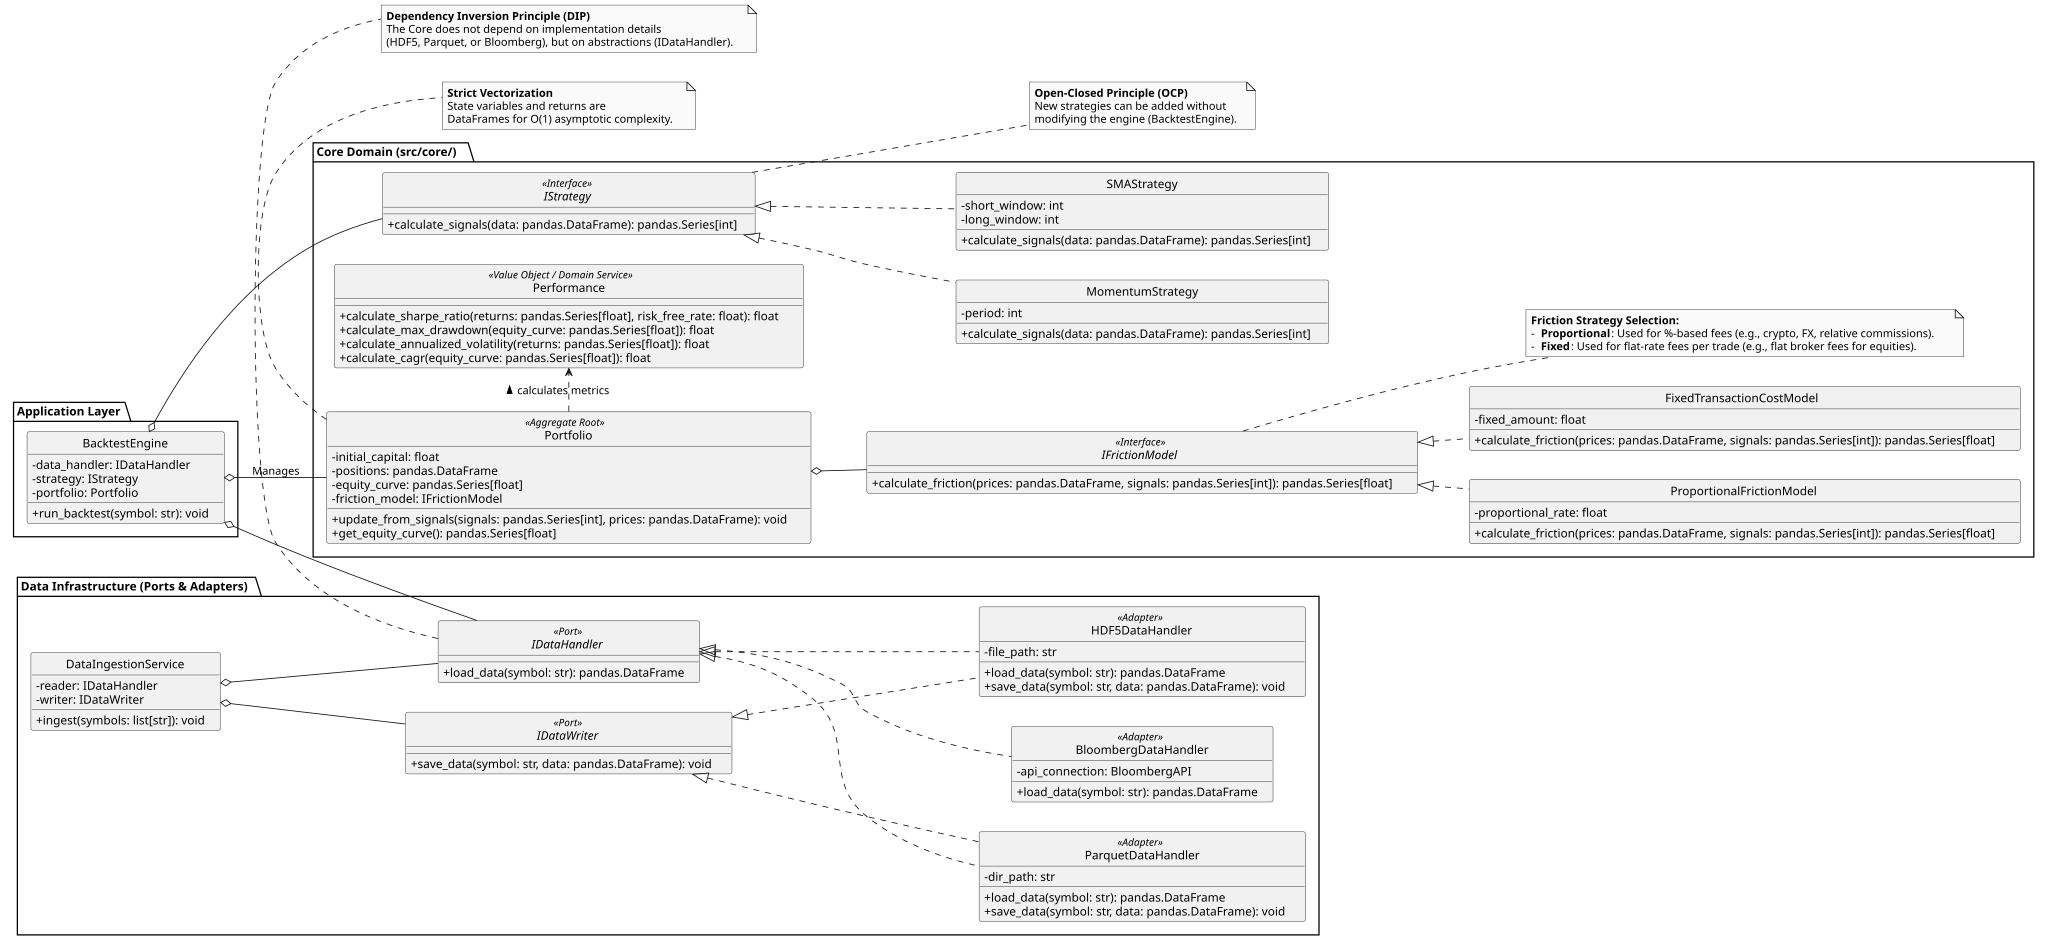
\includegraphics[width=\linewidth,height=14cm,keepaspectratio]{../architecture/class_diagram.pdf}
    \caption{Class Diagram of the Core Architecture}
    \label{fig:class_diagram}
\end{figuresrswide}
\vspace*{\fill}
\end{landscape}
The main components of the system and their fundamental methods span three architectural layers:

\subsection{Application Layer}
\begin{itemize}
    \item \textbf{\texttt{BacktestEngine}}: Acts as the central orchestrator. It encapsulates the injected dependencies (\texttt{IDataHandler}, \texttt{IStrategy}, \texttt{Portfolio}). Its \texttt{run\_backtest(symbol: str)} method coordinates the complete lifecycle: it invokes data loading, passes the \texttt{DataFrame} to the strategy to obtain signals, and delegates state updating and financial calculation to the portfolio.
\end{itemize}

\subsection{Core Domain}
\begin{itemize}
    \item \textbf{\texttt{Portfolio}}: Serves as the Aggregate Root. It maintains immutable state variables in matrix form: initial capital (\texttt{initial\_capital}), holdings (\texttt{positions}), and the value curve (\texttt{equity\_curve}). Its primary method, \texttt{update\_from\_signals(signals, prices)}, crosses trading signals with market returns and applies the injected friction model to generate the historical trajectory. It concludes by exposing the results via \texttt{get\_equity\_curve()}.
    
    \item \textbf{\texttt{IStrategy} and Concrete Strategies}: Base interface defining the pure contract \texttt{calculate\_signals(data) \allowbreak -> Series}. Implementations such as \textbf{\texttt{SMAStrategy}} (with state parameters \texttt{short\_window} and \texttt{long\_window}) or \textbf{\texttt{MomentumStrategy}} (with parameter \texttt{period}) materialize the algorithmic logic. This guarantees the Open-Closed Principle (OCP), allowing the array of strategies to scale without altering the main engine.
    
    \item \textbf{\texttt{IFrictionModel}}: Defines the contract \texttt{calculate\_friction(prices, \allowbreak signals) \allowbreak -> Series} to deduct transactional costs in a vectorized manner. It is materialized in specialized classes like \textbf{\texttt{ProportionalFrictionModel}} (applying a percentage rate, ideal for crypto or Forex) and \textbf{\texttt{FixedTransactionCostModel}} (applying an absolute cost per trade, typical in traditional stock brokerage).
    
    \item \textbf{\texttt{Performance}}: A stateless Domain Service, solely responsible for calculating risk and return metrics from time series. It exposes precise mathematical methods such as \texttt{calculate\_sharpe\_ratio()}, \texttt{calculate\_max\_drawdown()}, \texttt{calculate\_\allowbreak annualized\_\allowbreak volatility()}, and \texttt{calculate\_cagr()}.
\end{itemize}

\subsection{Data Infrastructure (Ports \& Adapters)}
\begin{itemize}
    \item \textbf{\texttt{IDataHandler} and \texttt{IDataWriter}}: Abstract ports defining \texttt{load\_data(symbol)} and \texttt{save\_data(symbol, data)}. They ensure the isolation of the predictive engine from persistence details (Dependency Inversion Principle - DIP).
    
    \item \textbf{Infrastructure Adapters}: Concrete implementations like \textbf{\texttt{HDF5\allowbreak DataHandler}} and \textbf{\texttt{Parquet\allowbreak DataHandler}} for massive hierarchical storage, or \textbf{\texttt{Bloomberg\allowbreak DataHandler}} for real-time or delayed ingestion from external APIs. Additionally, the \textbf{\texttt{DataIngestionService}} orchestrates the iterative fetching and persistence of multiple symbols.
\end{itemize}

\section{Execution Lifecycle}

The orchestration of the simulation follows a unidirectional and deterministic flow, designed to prevent the accidental alteration of state. This can be seen in the Sequence Diagram (Figure \ref{fig:sequence_diagram}).

\begin{figuresrs}
    \centering
    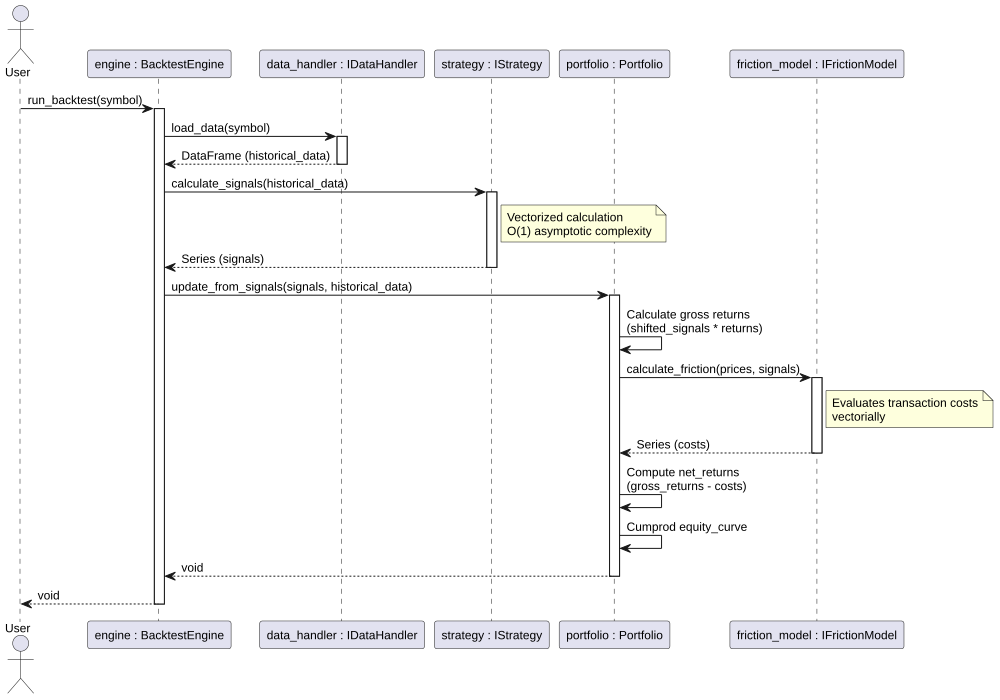
\includegraphics[width=\linewidth,height=17cm,keepaspectratio]{../architecture/sequence_diagram.pdf}
    \caption{Sequence Diagram of the Backtest Execution}
    \label{fig:sequence_diagram}
\end{figuresrs}

The flow is initiated by the user and delegated to the \texttt{BacktestEngine}. This orchestrator retrieves an immutable \texttt{DataFrame} of historical prices via \texttt{load\_data()} from the \texttt{IDataHandler} interface. Subsequently, it passes this structure to the \texttt{IStrategy} abstraction, which evaluates the market and returns an array of signals (e.g., \(+1\), \(0\), \(-1\)). Finally, \texttt{Portfolio} ingests both the prices and the signals in a single matrix operation.

\section{Vectorized Activity Pipeline}

To comply with the strict computational complexity requirement of \(\mathcal{O}(1)\) over massive financial arrays (avoiding any imperative \texttt{for} or \texttt{while} loops), the core of the \texttt{Portfolio} is designed as a purely mathematical conduit. Figure \ref{fig:activity_diagram} details this pipeline.

\begin{figuresrs}
    \centering
    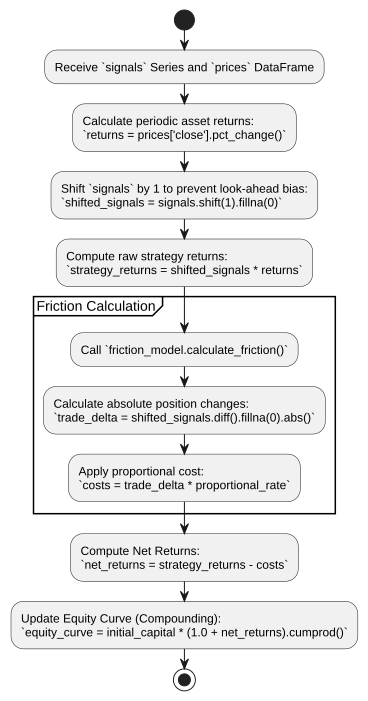
\includegraphics[width=0.6\linewidth]{../architecture/activity_diagram.pdf}
    \caption{Activity Diagram: Vectorized Pipeline in the Portfolio}
    \label{fig:activity_diagram}
\end{figuresrs}
\clearpage
Prior to the algorithmic execution, we establish the foundational mathematical definitions that govern the vectorized operations:

\begin{definition}[Simple Returns]
Let \( P_t \) denote the price of the asset at time \( t \). The discrete percentage return \( R_t \) is calculated as:
\begin{equation}
    R_t = \frac{P_t - P_{t-1}}{P_{t-1}}
\end{equation}
\end{definition}

\begin{definition}[Transaction Friction]
Let \( S_t \in \{-1, 0, 1\} \) be the trading signal at time \( t \) and \( c \) the proportional transaction cost. The friction penalty \( F_t \) incurred at time \( t \) is proportional to the absolute state transition:
\begin{equation}
    F_t = c \cdot | S_t - S_{t-1} |
\end{equation}
\end{definition}

\begin{definition}[Equity Curve]
Given the initial capital \( C_0 \), the strategy signals \( S_{t-1} \) (shifted to avoid look-ahead bias), and the friction \( F_t \), the net return \( \tilde{R}_t \) is \( \tilde{R}_t = S_{t-1} R_t - F_t \). The portfolio value \( E_T \) is defined as the cumulative product:
\begin{equation}
    E_T = C_0 \prod_{t=1}^{T} (1 + \tilde{R}_t)
\end{equation}
\end{definition}

The fundamental algorithmic steps applied to the DataFrame, guaranteeing performance, are:
\begin{enumerate}
    \item \textbf{Returns Calculation:} Native percentage differentiation of the price series.
    \item \textbf{Signal Shifting:} The input signals are mandatorily shifted one time unit forward (\texttt{shift(1)}) to avoid look-ahead bias, ensuring that the investment state at time \(t\) is only executed with the return observed at \(t+1\).
    \item \textbf{Friction Calculation:} The absolute differential of the positions is evaluated through arrays (\texttt{diff().abs()}) to financially penalize only the state transitions, subtracting the associated costs in bulk.
    \item \textbf{Equity Curve:} The continuous cumulative product (\texttt{cumprod()}) is applied to the net returns, achieving the complete evaluation of the historical path in a single native call to the low-level C routines of Pandas/NumPy.
\end{enumerate}

\chapter{Implementation and Vectorization}

\section{Vectorization over Iteration}
Explain the strict paradigm of avoiding \texttt{for} or \texttt{while} loops. Detail how \texttt{pandas} and \texttt{NumPy} were used to achieve $\mathcal{O}(1)$ asymptotic complexity for array operations across time-series data.

\section{Structured Programming}
Detail the adherence to academic structured programming paradigms, including the absolute prohibition of control flow interruption statements like \texttt{break} or \texttt{continue}.

\section{Friction Models}
Describe the implementation of the \texttt{IFrictionModel} for transaction costs calculation without loops, strictly using dataframe shift operations.

\chapter{Results and Conclusions}

\section{Backtest Execution Analysis}
Analysis of the performance and execution time. Showcase the output of the Jupyter notebook visualizations (\texttt{matplotlib} and \texttt{plotly}) plotting the \textit{Equity Curve}.

\section{Conclusions}
Summary of the project's achievements against its initial goals in terms of software architecture, algorithmic efficiency, and mathematical rigor.

\section{Future Work}
Potential improvements, such as adding new statistical models, expanding the framework to multi-asset portfolios, or integrating real-time live trading connectivity.

\subsection{Memory Optimization with NumExpr}

While the current architecture leverages \texttt{NumPy} and \texttt{pandas} to achieve \(\mathcal{O}(1)\) time complexity through vectorization, standard \texttt{NumPy} operations evaluate expressions sequentially and allocate intermediate arrays in memory. For instance, calculating a complex sequence like \( A \times B - C \) creates temporary memory buffers for each sub-operation before yielding the final result.

The current project scope does not utilize \texttt{numexpr}, a high-performance numerical expression evaluator. For the existing daily or minute-resolution backtests, standard vectorization provides sufficient speed without introducing additional third-party dependencies. However, as future work, integrating \texttt{numexpr} (or leveraging \texttt{pandas.eval()}) is highly recommended when scaling the engine to process high-frequency, tick-level data across thousands of simultaneous assets. \texttt{numexpr} evaluates complex algebraic expressions element-wise in C without allocating intermediate arrays and dynamically distributes the workload across multiple CPU cores. This architectural upgrade would significantly optimize the memory footprint (Space Complexity) and further reduce the computational constant factors of the backtesting pipeline.


\newpage
\nocite{*}
\printbibliography[heading=bibintoc, title={References}]

\end{document}
